\documentclass[10pt]{article}

\def\Type{LessonCaelan}
\def\TypeNum{Lesson 8}
\def\TypeTitle{Chain Rule\\Notes to Instructors }
\def\Semester{Fall 2021} %Not Used 
\def\Course{MATH 1190 \& 1210}
\def\Targets{ {\bf\color{ForestGreen}D2} }

\usepackage{preambleDJ}




%%%%%%%%%%%% BEGIN DOCUMENT %%%%%%%%%%%%%%%
%%%%%%%%%%%% BEGIN DOCUMENT %%%%%%%%%%%%%%%
%%%%%%%%%%%% BEGIN DOCUMENT %%%%%%%%%%%%%%%
%%%%%%%%%%%% BEGIN DOCUMENT %%%%%%%%%%%%%%%
%%%%%%%%%%%% BEGIN DOCUMENT %%%%%%%%%%%%%%%



\begin{document}

\pagestyle{otherpages}
\thispagestyle{firstpage}
\vs{.75}
\lt
\enumC{
\item[D2:] Computing Derivatives
\itemC{
 \item Apply the chain rule to take the derivative. (\target{D2})
\item Determine the order of applying differentiation rules when multiple rules are to be applied. (\target{D2})
}
}


~\\
\lg Students will be able to...
\enum{
\item Compose two functions
\item Identify which is the ``inner" and `outer" functions in a composition.
\item Apply the Chain Rule using Prime/Lagrange notation.
\item Utilize Leibniz notation to interpret the sign(s) of individual derivatives in the Chain Rule in context.
\item Identify which derivative technique should be used to start a problem when derivative requires more than one technique.
\item Utilize graphical information or tables of data to determine the value of derivatives using the Chain Rule.
}

%\feed Due to a technical problem in F24, we were not able to collect feedback for this lesson.


 \hand
 \itemI{
 \item Page 1 is designed to increase confidence and competence to a) compose functions when given individual functions and b) identify inner/outer functions when given the composition.
 \item Exercises A  provides practice implementing Chain Rule on functions from p. 1 where inner/outer functions have been identified.
 \item Exercise B scaffolds students to deal with a challenging derivative that requires Product, Quotient and Chain Rule
 \itemI{
 \item Part a) requires students to both identify inner/outer functions and implement Chain Rule.  
 \item Part b) requires the Product Rule in addition to Chain Rule. Work from a) should be utilized in b). 
 \item Part c) requires Quotient and Product rule in addition to Chain Rule. Work from b) should be utilized in c)
  }
  \item Leibniz notation for the Chain Rule is introduced and Exercise C provides practice using Leibniz notation to interpret various derivatives in context
  \item Extra Practice1 is a terrific conceptual problem that requires students to understand structure of Chain Rule but evaluate each derivative from provided graphical information.
  \item Extra Practice 2 is a challenging, un-scaffolded question that requires Chain, Product and Quotient Rules.  If a student can complete this problem, they will have very good understanding of these techniques.
  \item Extra Practice 3 is more practice with Leibniz notation and practice interpreting various derivatives in context.
 }

\core Warmup Exercises 1 and 2, Exercises A, B, and C.

\newpage

{\bf \blue{Outer \& Inner Functions}}\\
 {\bf\color{blue}Warm-up Exercise 1.} Suppose $h(x) = x^{\frac{3}{2}}$ and $j(x) = x^2 - x+1$.

\enumA{
    \item Define $(h\circ j)(x) = h(j(x))$. Note that $(h\circ j)(x)$ is a \textit{composite function}, where $h$ is the ``outside'' or ``outer'' function and $j$ is the ``inside'' or ``inner'' function. Write a formula for $(h\circ j)(x)$.
    
\sol{
$\ds (h\circ j)(x) = h(j(x))=h(x^2-x+1)=(x^2-x+1)^{3/2}$
}

    
    \item  Define $(j\circ h)(x) = j(h(x))$.  Now $(j \circ h)$ is also a \textit{composite function}. This time, $j$ is the ``outside'' or ``outer'' function and $h$ is the ``inside'' or ``inner'' function. Write a formula for $(j\circ h)(x)$.
    
\sol{
$\ds (j\circ h)(x) = j(h(x))= j(x^{3/2})=(x^{3/2})^2-x^{3/2}+1=x^3-x^{3/2}+1$
}

}

{\bf\color{blue}Warm-up Exercise 2.} The following are compositions of functions. Decide what the outer function $f$ and inner function $g$ are, testing your choices by finding $(f\circ g)(x)=f(g(x))$ in the space provided.\\

\enumA{
\item  \begin{tabular}{p{1.25in}ll}  $(x^2+2x-1)^4$ & {\large outer $f(x)=$\unline{1}{ \blue{$x^4$} }{.25}} &\qquad {\large inner $g(x)=$\unline{1}{\blue{$x^2+2x-1$}}{.25}} \\   \end{tabular}~\\
\sol{
$\ds f(g(x))=f(x^2+2x-1)=(x^2+2x-1)^4$
}
\vs{.3}
\item   \begin{tabular}{p{1.25in}ll} $\sqrt{e^x+1}$ \qquad & {\large outer $f(x)=$\unline{1}{\blue{$\sqrt{x}$}}{.25}} &\qquad {\large inner $g(x)=$\unline{1}{\blue{$e^x+1$}}{.25}} \\   \end{tabular}~\\
\sol{
$\ds f(g(x))=f(e^x+1)=\sqrt{e^x+1}$
}
\vs{.3}
\item  \begin{tabular}{p{1.25in}ll} $e^{\sqrt{x}}+1$  & {\large outer $f(x)=$\unline{1}{\blue{$e^x+1$}}{.25}} &\qquad {\large inner $g(x)=$\unline{1}{\blue{$\sqrt{x}$}}{.25}} \\   \end{tabular}~\\
\sol{
$\ds f(g(x))=f(\sqrt{x})=e^{\sqrt{x}}+1$
}

}
%\item $(x^2+2x-1)^4$ \,\hfill 
%    {\large outer $f(x)=$\unline{1}{}{.25}}
%   \hfill
%    {\large inner $g(x)=$\unline{1}{}{.25}}
   % \\[0.75in]
%}

%\item $\sqrt{e^x+1}$ \,\hfill 
%    {\large outer $f(x)=$\unline{1}{}{.25}}
%\hfill
%    {\large inner $g(x)=$\unline{1}{}{.25}}
%    \\[0.75in]
%    
%
%\item $e^{\sqrt{x}}+1$ \,\hfill 
%    {\large outer $f(x)=$\unline{1}{}{.25}}
%   \hfill
%    {\large inner $g(x)=$\unline{1}{}{.25}}
%    \\[0.75in]



%\end{document} %end document here for pre-class assignment

%%%%%%%%%
\newpage%
%%%%%%%%%



{\bf \blue{ Chain Rule: Prime Notation or Lagrange Notation}}\mod


The {\bf Chain Rule} gives a way to compute derivatives of compositions of functions. \\
{\em Key Idea:} \\
\blue{Look for function ``inside" another function" to use this technique}
\vs{.3}

{\bf Prime notation:} If $g$ is differentiable at $x$ and $f$ is differentiable at $g(x)$, then the composite function $f \circ g$ defined by $(f \circ g)(x)=f(g(x))$ is differentiable at $x$ and $(f \circ g)'$ is given by the formula \\\\

\hs{.5}$\ds \frac{d}{dx}\left[ (f\circ g)(x)\right]=$  \blue{$\ds \frac{d}{dx} f(g(x))$ =Deriv of ``outer" $\times$ deriv of ``inner" $=\underbrace{f^{\prime}(g(x))}_{deriv \;outer} \cdot \underbrace{g^{\prime}(x)}_{deriv\;inner}$} 
\\\\


{\bf\color{blue} GOAL:} The following 2 exercises build skills needed in learning target {\bf\color{ForestGreen}D2}, an important learning target in MATH 1190 \& 1210. {\bf\color{ForestGreen}D2} prompts typically involve functions represented algebraically, graphically, or tabularly, and using all three of the product, quotient, and chain rules.


{\exercise{\color{ForestGreen}D2}} Use the derivative rules on the previous page to find the following derivatives:

\begin{enumerate}
\item[(a)]$\displaystyle\frac{d}{dx}\left[ (x^2+2x-1)^4 \right]$\\
\mpageT{.5}{.5}{
\sol{
\itemNIN{
\item Outer: $f(x)=x^4$
\item Inner: $g(x)=x^2+2x-1$
\item $\ds f^{\prime}(x)=4x^3$
\item $\ds f^{\prime}(g(x))=4(x^2+2x-1)^3$
\item $\ds g^{\prime}(x)=2x+2$
}
}
}{\blue{\vs{.2}
\al{
 \frac{d}{dx}\left[ (x^2+2x-1)^4 \right]&=f^{\prime}(g(x))\cdot g^{\prime}(x)\\\\
 &=\underbrace{4(x^2+2x-1)^3}_{deriv\; outer}\cdot \underbrace{(2x+2)}_{deriv\; inner}
}
}
}
\item[(b)] $\displaystyle \frac{d}{dx}\left[ \sqrt{e^x+1} \right]$

\mpageT{.5}{.5}{
\sol{
\itemNIN{
\item Outer: $f(x)=\sqrt{x}=x^{1/2}$
\item Inner: $g(x)=e^x+1$
\item $\ds f^{\prime}(x)=\frac{1}{2}x^{-1/2}$
\item $\ds f^{\prime}(g(x))=\frac{1}{2}(e^x+1)^{-1/2}$
\item $\ds g^{\prime}(x)=e^x+0$
}
}
}{\blue{\vs{.2}
\al{
 \frac{d}{dx}\left[ \sqrt{e^x+1} \right]&=f^{\prime}(g(x))\cdot g^{\prime}(x)\\
 &=\underbrace{\frac{1}{2}(e^x+1)^{-1/2}}_{deriv\; outer}\cdot \underbrace{e^x}_{deriv\; inner}
}
}
}
\item[(c)] $\displaystyle \frac{d}{dx}\left[ e^{\sqrt{x}}+1 \right]$

\mpageT{.5}{.5}{
\sol{
\itemNIN{
\item Outer: $f(x)=\sqrt{x}=e^x+1$
\item Inner: $g(x)=\sqrt{x}=x^{1/2}$
\item $\ds f^{\prime}(x)=e^x+0$
\item $\ds f^{\prime}(g(x))=e^{\sqrt{x}}$
\item $\ds g^{\prime}(x)=\frac{1}{2}x^{-1/2}$
}
}
}{\blue{\vs{.2}~\\
\al{
\frac{d}{dx}\left[ e^{\sqrt{x}}+1 \right]&=f^{\prime}(g(x))\cdot g^{\prime}(x)\\
 &=\underbrace{e^{\sqrt{x}}}_{deriv\; outer}\cdot \underbrace{\frac{1}{2}x^{-1/2}}_{deriv\; inner}
}
}
}

\end{enumerate}


%%%%%%%%%
\newpage%
%%%%%%%%%


\exercise{\color{ForestGreen}D2} Find the following derivatives:

\begin{enumerate}
\item[(a)] $\displaystyle \frac{d}{dy}\left[ (y^2-1)^{3/2} \right]$

\mpageT{.5}{.5}{
\sol{
\itemNIN{
\item Outer: $f(y)=y^{3/2}$
\item Inner: $g(x)=y^2-1$
\item $\ds f^{\prime}(y)=\frac{3}{2}y^{1/2}$
\item $\ds f^{\prime}(g(y))=\frac{3}{2}(y^2-1)^{1/2}$
\item $\ds g^{\prime}(y)=2y-0$
}
}
}{\blue{\vs{.2}
\al{
\frac{d}{dy}\left[ (y^2-1)^{3/2} \right]&=f^{\prime}(g(y))\cdot g^{\prime}(y)\\
 &=\underbrace{\frac{3}{2}(y^2-1)^{1/2}}_{deriv\; outer}\cdot \underbrace{2y}_{deriv\; inner}
}
}
}


\item[(b)] $\displaystyle\frac{d}{dy}\left[ y(y^2-1)^{3/2} \right] \blue{= \frac{d}{dy}\left[f(y)\cdot g(y)\right]}$ \blue{where $f(y)=y$ and $g(y)=(y^2-1)^{3/2}$.}\\
\sol{
We have two functions multiplied together:
$$ \frac{d}{dy}\left[ y(y^2-1)^{3/2} \right] = \frac{d}{dy}\left[f(y)\cdot g(y)\right]$$
where $f(y)=y$ and $g(y)=(y^2-1)^{3/2}$. So we must start with the {\em product rule}. 

Informally: {\em Deriv first $\times$ second $+$ first $\times$ deriv second}\\
Formally:  
\al{
 \frac{d}{dy}\left[f(y)\cdot g(y)\right]&=f^{\prime}(y)\cdot g(y)+f(y)\cdot g^{\prime}(y)
 \intertext{$f(y)=y \Rightarrow f^{\prime}(y)=1$ and $g(y)=(y^2-1)^{3/2}\Rightarrow g^{\prime}(y)=\frac{3}{2}(y^2-1)^{1/2}\cdot 2y$ {\bf (from part a))}}
 &=1\cdot (y^2-1)^{3/2}+y\cdot \frac{3}{2}(y^2-1)^{1/2}\cdot 2y
 }
}

\item[(c)] $\displaystyle\frac{d}{dy}\left[ \frac{y(y^2-1)^{3/2}}{5y+1} \right]$\blue{$\ds =\frac{d}{dy}\left[\frac{f(y)}{g(y}\right]$ where $f(y)=y(y^2-1)^{3/2}$ and $g(y)=5y+1$.}\\
\sol{
We have two functions divided which means we need to start with the {\em quotient rule}.

Informally: $\ds \frac{\text{lo}\;\text{d hi} - \text{hi}\;\text{d lo}}{\text{lo lo}}$

Formally:
\al{
\frac{d}{dy}\left[\frac{f(y)}{g(y}\right]&=\frac{f^{\prime}(y)g(y)-f(y)g^{\prime}(y)}{[g(y)]^2}
\intertext{$f(y)=y(y^2-1)^{3/2}$. This is the function from {\bf part b)}. \vs{.1}\newline
We use the result we've already found: $\ds f^{\prime}(y)=1\cdot (y^2-1)^{3/2}+y\cdot \frac{3}{2}(y^2-1)^{1/2}\cdot 2y$. \vs{.1}\newline
Also, $g(y)=5y+1\Rightarrow g^{\prime}(y)=5+0$}
&=\frac{\left(1\cdot (y^2-1)^{3/2}+y\cdot \frac{3}{2}(y^2-1)^{1/2}\cdot 2y \right)(5y+1)-y(y^2-1)^{3/2}(5+0)}{(5y+1)^2}
}
}


\end{enumerate}


%%%%%%%%%
\newpage%
%%%%%%%%%



{\bf \blue{ Chain Rule: Leibnitz Notation}}

The {\bf Chain Rule} gives a way to compute derivatives of compositions of functions. Please fill in the blanks in the statement of the Chain Rule {\it using Leibniz notation} below. \\

{\bf Leibniz notation:} If $y$ is a differentiable function of $u$ and $u$ is a differentiable function of $x$, then \\

\hs{.5}$\ds \frac{dy}{dx}=\blue{\frac{dy}{du}\cdot\frac{du}{dx}}$\\
\nti{
This makes sense if we abuse notation just a bit.  
$$\frac{dy}{du}\cdot\frac{du}{dx}=\frac{dy}{\cancel{du}}\cdot\frac{\cancel{du}}{dx}=\frac{dy}{dx}$$
}

\exercise{\color{ForestGreen}D2} Let $w$ represent the weight (in pounds) of an average infant. The weight of an infant can be regarded as a function of the height $h$ (in inches) of the infant, and height can further be regarded as a function of age $t$ (in months):
\[w=w(h(t))\]
\enumA{
\item What are the units of measurement of $\dfrac{dw}{dt}$,  $\dfrac{dh}{dt}$, and $\dfrac{dw}{dh}$?\\

{\Large \,\hfill $\dfrac{dw}{dt}:$\unline{1.5}{ \blue{$\ds \frac{\text{pounds}}{\text{month}}$} }{.4} \hfill $\dfrac{dh}{dt}:$\unline{1.5}{\blue{$\ds \frac{\text{inches}}{\text{month}}$}}{.4} \hfill $\dfrac{dw}{dh}:$\unline{1.5}{ \blue{$\ds \frac{\text{pounds}}{\text{inch}}$} }{.4} \hfill\,}\\

\mpageT{.5}{.5}[\hs{.3}]{
\item Given $w=w(h(t))$, use Leibniz notation to write down the derivative of $w$ with respect to $t$. Your answer should involve $\dfrac{dw}{dt}$,  $\dfrac{dh}{dt}$, and $\dfrac{dw}{dh}$.
\sol{
$$\frac{dw}{dt}=\frac{dw}{dh}\cdot\frac{dh}{dt}$$
}
}{
\item Is $\dfrac{dw}{dh}$ positive, negative, or zero? Give a description of the relationship \& a mathematical justification incorporating the context of this problem while explaining your answer. ({\bf NOTE:} explanations are of the utmost importance in this class. We care more about your thought process than your final answer, so please make sure your answers are well-supported!)
\sol{
\itemI{
\item We expect an infant to gain weight over time, so $\ds \frac{dw}{dt}=(+)$.
\item We also expect an infant to gain height over time, so $\ds \frac{dh}{dt}=(+)$.
\item Using the Leibniz version of the Chain Rule, we know
\al{
\frac{dw}{dt}&=\frac{dw}{dh}\cdot\frac{dh}{dt}\\
(+)&=\frac{dw}{dh}\cdot (+)\\
\frac{(+)}{(+)}&=\frac{dw}{dh}
}
Thus $\ds \frac{dw}{dh}=(+)$ which means the infants weight increases as height increases.
}
}
}
}


%%%%%%%%%
\newpage%
%%%%%%%%%


%\,
%
%\vspace{-0.5in}

%
{\bf\color{blue}Extra Practice 1.}
%
\reversemarginpar\marginnote{\fbox{\bf\color{ForestGreen}D2}} 
%
Let $k(x)=f(g(x))$, where $f$ and $g$ are functions whose graphs are shown below. What is the value of $k'(5)$?  \\
\mpageT{.4}{.6}{
\begin{center}
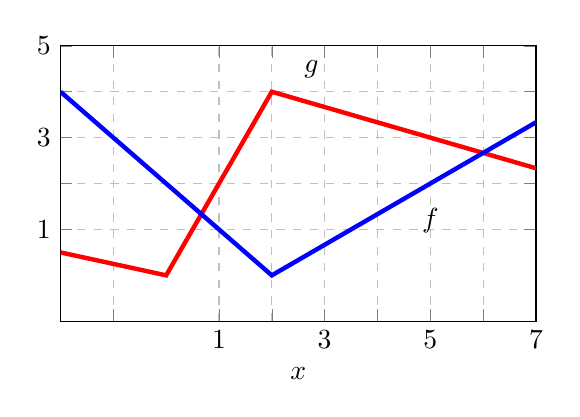
\begin{tikzpicture}
  \begin{axis}[
    xlabel={$x$},
    xtick       = {-2,-1,1,2,3,4,5,6,7},
    xticklabels = { , ,$1$, ,$3$ , ,$5$ , , $7$},
    ytick       = {-1,1,2,3,4,5},
    yticklabels = { ,$1$, ,$3$ , ,$5$ },
    samples     = 320,
    domain      = -3.5:3.5,
    %restrict y to domain=-2.5:4.5,
    xmin = -2, xmax = 7,
    ymin = -1, ymax = 5,
    width = 3in, height = 2in,
    grid=both, grid style=dashed
  ]
  \draw[red,ultra thick] (-2,0.5) -- (0,0) -- (2,4) -- (8,2);
  \node at (2.75,4.5) {$g$};
  \draw[blue,ultra thick] (-2,4) -- (2,0) -- (8,4);
  \node at (5,1.2) {$f$};
\end{axis}
\end{tikzpicture}
\end{center}
}{
\sol{
\al{
k^{\prime}(5)&=f^{\prime}(g(5))\cdot g^{\prime}(5)
\intertext{From the graph, $g(5)=3$}
&=f^{\prime}(3)\cdot g^{\prime}(5)
\intertext{From the graph, slope of $f$ at $x=3$ is $\ds\frac{2}{3}$. Thus $\ds f^{\prime}(3)=\frac{2}{3}$}
&=\frac{2}{3}\cdot g^{\prime}(5)
\intertext{From graph, slope of $g$ at $x=5$ is $-\dfrac{1}{3}$.  Thus $\ds g^{\prime}(5)=-\frac{1}{3}$}
&=\frac{2}{3}\cdot -\frac{1}{3}\\
&=-\frac{2}{9}
}
}
}

{\bf\color{blue}Extra Practice 2.}
%
\reversemarginpar\marginnote{\fbox{\bf\color{ForestGreen}D2}} 
%
Find the following derivative: $\dfrac{d}{dx}\left[\sqrt{\dfrac{1+x^2e^x}{1-e^x}} \right]$

\sol{ This is a challenging question! 
We have a "function inside of a function". The ``outer" function is $f(x)=\sqrt{x}=x^{1/2}$. The ``inner" function is $\ds g(x)=\frac{1+x^2e^x}{1-e^x}$.\\
}
\mpageT{.6}{.4}[\hs{.1}]{\blue{
\al{
\frac{d}{dx}\left[\sqrt{\dfrac{1+x^2e^x}{1-e^x}} \right]&=\frac{d}{dx}\left[f(g(x))\right]\\
&=f^{\prime}(g(x))\cdot g^{\prime}(x)\\
&=\frac{1}{2}(g(x))^{-1/2}\cdot g^{\prime}(x)\\
&=\frac{1}{2}\left(\frac{1+x^2e^x}{1-e^x} \right)^{-1/2}\cdot g^{\prime}(x)\\\\\\\\\\
&=\frac{1}{2}\left(\frac{1+x^2e^x}{1-e^x} \right)^{-1/2}\cdot \left( \frac{hi^{\prime}\cdot lo-hi\cdot lo^{\prime}}{\left[lo\right]^2} \right)\\
&=\frac{1}{2}\left(\frac{1+x^2e^x}{1-e^x} \right)^{-1/2}\cdot \left( \frac{hi^{\prime}\cdot (1-e^x)-hi\cdot (-e^x)}{\left[1-e^x\right]^2} \right)\\\\
}
}
}{
\blue{
\vs{.65}
$\leftarrow$ We have $\ds f(x)=x^{1/2}$, so $\ds f^{\prime}(x)= \frac{1}{2}x^{-1/2}$\\
$\leftarrow$ $\ds g(x)=\frac{1+x^2e^x}{1-e^x}$ so we substitute for $g$\vs{.15}\\
$\leftarrow$ For the next step, we need to find $g^{\prime}(x)$. Since $\ds g(x)=\frac{1+x^2e^x}{1-e^x}$, we have two functions divided by each other. We will need to use the {\em Quotient Rule} where $hi(x)= 1+x^2e^x$ and $lo(x)=1-e^x$.\\\\
$\leftarrow$ $lo(x)=1-e^x$ and thus $$lo^{\prime}(x)=0-e^x=-e^x$$
$\leftarrow$ $hi(x)=1+x^2e^x$ and we must use the {\em Product Rule} to find $hi^{\prime}(x)$. In particular
$$hi^{\prime}(x)=0+\left(2x\cdot e^x +x^2 \cdot e^x\right)$$
}
}
\blue{
$$\hs{.6}=\frac{1}{2}\left(\frac{1+x^2e^x}{1-e^x} \right)^{-1/2}\cdot \left( \frac{\left(2x\cdot e^x +x^2 \cdot e^x\right)\cdot (1-e^x)-(1+x^2e^x)\cdot (-e^x)}{\left[1-e^x\right]^2} \right)$$
}

{\bf\color{blue}Extra Practice 3.}
%
\reversemarginpar\marginnote{\fbox{\bf\color{ForestGreen}D2}} 
%
The flux $F$ of blood through a vessel -- that is, the volume of blood per unit time that flows past a given point -- can be regarded as a function of the radius $R$ of the vessel. In particular, when $R$ changes, so too does $F$.

\begin{enumerate}
\item[(a)] Assuming $F$ is measured in $\dfrac{mm^3}{sec}$, $R$ is measured in $mm$, and $t$ is measured in $sec$, what are the units of the following derivatives?\\
\,
\hfill
{\large $\dfrac{dF}{dt}$:\unline{1.25}{ \blue{$\ds \frac{mm^3/sec}{sec}=\frac{mm^3}{sec^2}$} }{.4}}
\hfill
{\large $\dfrac{dF}{dR}$: \unline{1.25}{ \blue{$\ds \frac{mm^3/sec}{mm}=\frac{mm^2}{sec}$} }{.4}}
\hfill
{\large $\dfrac{dR}{dt}$: \unline{1.25}{  \blue{$\ds \frac{mm}{sec}$} }{.4}}
\hfill
\,\\[0.2in]

\item[(b)] When the human body experiences a drop in blood pressure -- due to, for example, blood loss or dehydration -- it creates and distributes a hormone called angiotensin to raise blood pressure by decreasing blood vessels' radii. How are $\dfrac{dF}{dt}$ and $\dfrac{dF}{dR}$ related once angiotensin has been created and distributed?\\

\mpageT{.4}{.6}{
\begin{enumerate}
\item[A.] They are the same.
\item[B.] Both are positive.
\item[C.] Both are negative.
\item[D.] One is positive and one is negative.
\item[E.] none of the other answers\\
\end{enumerate}
}{
\sol{
\itemI{
\item We're told that  the hormone called angiotensin to {\em  raises blood pressure by decreasing blood vessels' radii}. This means $\ds \frac{dR}{dt}=(-)$ when angiotensin is distributed in the blood.
\item Leibniz notation of the Chain Rule is 
\al{
\frac{dF}{dt}&=\frac{dF}{dR}\cdot \frac{dR}{dt}\\
\frac{dF}{dt}&=\frac{dF}{dR}\cdot (-)
}
\item If $\ds \frac{dF}{dR}=(+)$ then we have
$$\frac{dF}{dt}=(+)\cdot (-)$$ and it is the case that $\ds \frac{dF}{dt}=(-)$, i.e. the opposite sign of $\dfrac{dF}{dR}$
\item On the other hand, if $\ds \frac{dF}{dt}=(+)$ then we have
\al{
(+)&=\frac{dF}{dR}\cdot (-)\\
\frac{(+)}{(-)}&=\frac{dF}{dR}
}
and $\ds \frac{dF}{dR}=(-)$ which is again the opposite sign of $\dfrac{dF}{dt}$. 
\item Thus the best choice is {\bf D. One is positive and one is negative}.
}
}
}


\end{enumerate}


\end{document}
